\section{The Silicon Tracker}
\label{sec:tracker}

At the heart of CMS is one of the world's largest silicon detectors: the silicon tracker.
The main goal of the silicon tracker to very precisely measure the hits from outgoing charged particles as they pass through this subdetector.
The tracker consists of two types of pure silicon detectors: the pixel detector and the strip detector, each of which is described in detail below.
% , and are absolutely necessary to \emph{track} the decay products from $pp$ collisions.

\subsection{The Pixel Detector}
\label{subsec:pixel}

The innermost part of the silicon tracker is the pixel detector which is , the closest subdetector of CMS to the IP, is the pixel detector made of minuscule silicon ``pixels'', as shown in Fig.~\ref{fig:tracker_real} (Left, pink).
Each pixel is 100$\mu$m x 150$\mu$m in size and, with 66 million of them, they altogether cover a sensitive area of 1.9 m$^2$. 
The pixel detector has the highest particle flux out of any other subdetector, since it sits only 8 cm away from the beam pipe:
it receives around 10 million particles per cm$^2$ per second.
The pixel detector is made of three cylindrical layers and two endcaps that surround the beam pipe.
Impressively, the pixel detector has around 6,000 connections (channels) per cm$^2$.

During the 2016 LHC running period, the silicon tracker 


REFERENCING THE CMS DETECTOR
How Hualin has it:
C. Collaboration, "the CMS Experiment at the CERN LHC," \textit{Journal of Instrumentation}, vol. 3, p. S08004, 2008.
Compare the above to what gets printed out when you get bibtex working!

\subsection{The Strip Detector}
\label{subsec:strip}

The outer part of the Silicon Tracker is called the strip detector, which has 10 million detector strips spread across 10 cylindrical layers.
The first 4 layers belong to the tracker inner barrel (TIB) and the remaining 6 layers belong to the tracker outer barrel (TOB), Fig.~\ref{fig:tracker_real} (Left, green and blue, respectively). 
Both the TIB and TOB have two endcaps associated with them, the TID and TEC, respectively.
Accounting for all of its components, the strip detector is sensitive to 200 m$^2$.
Fig.~\ref{fig:tracker_xs} gives a clearly-labelled transverse illustration of the pixel and strip detectors.
% It functions similarly to the pixels in that 
% It also has has slightly worse resolution than the pixel detector.
% Both the pixel and strip trackers have barrel and endcap components for nearly hermetic coverage around the beam pipe.
%%%%%%%%%%%%%%%%%%%%
\begin{figure}[pbth]
\centering
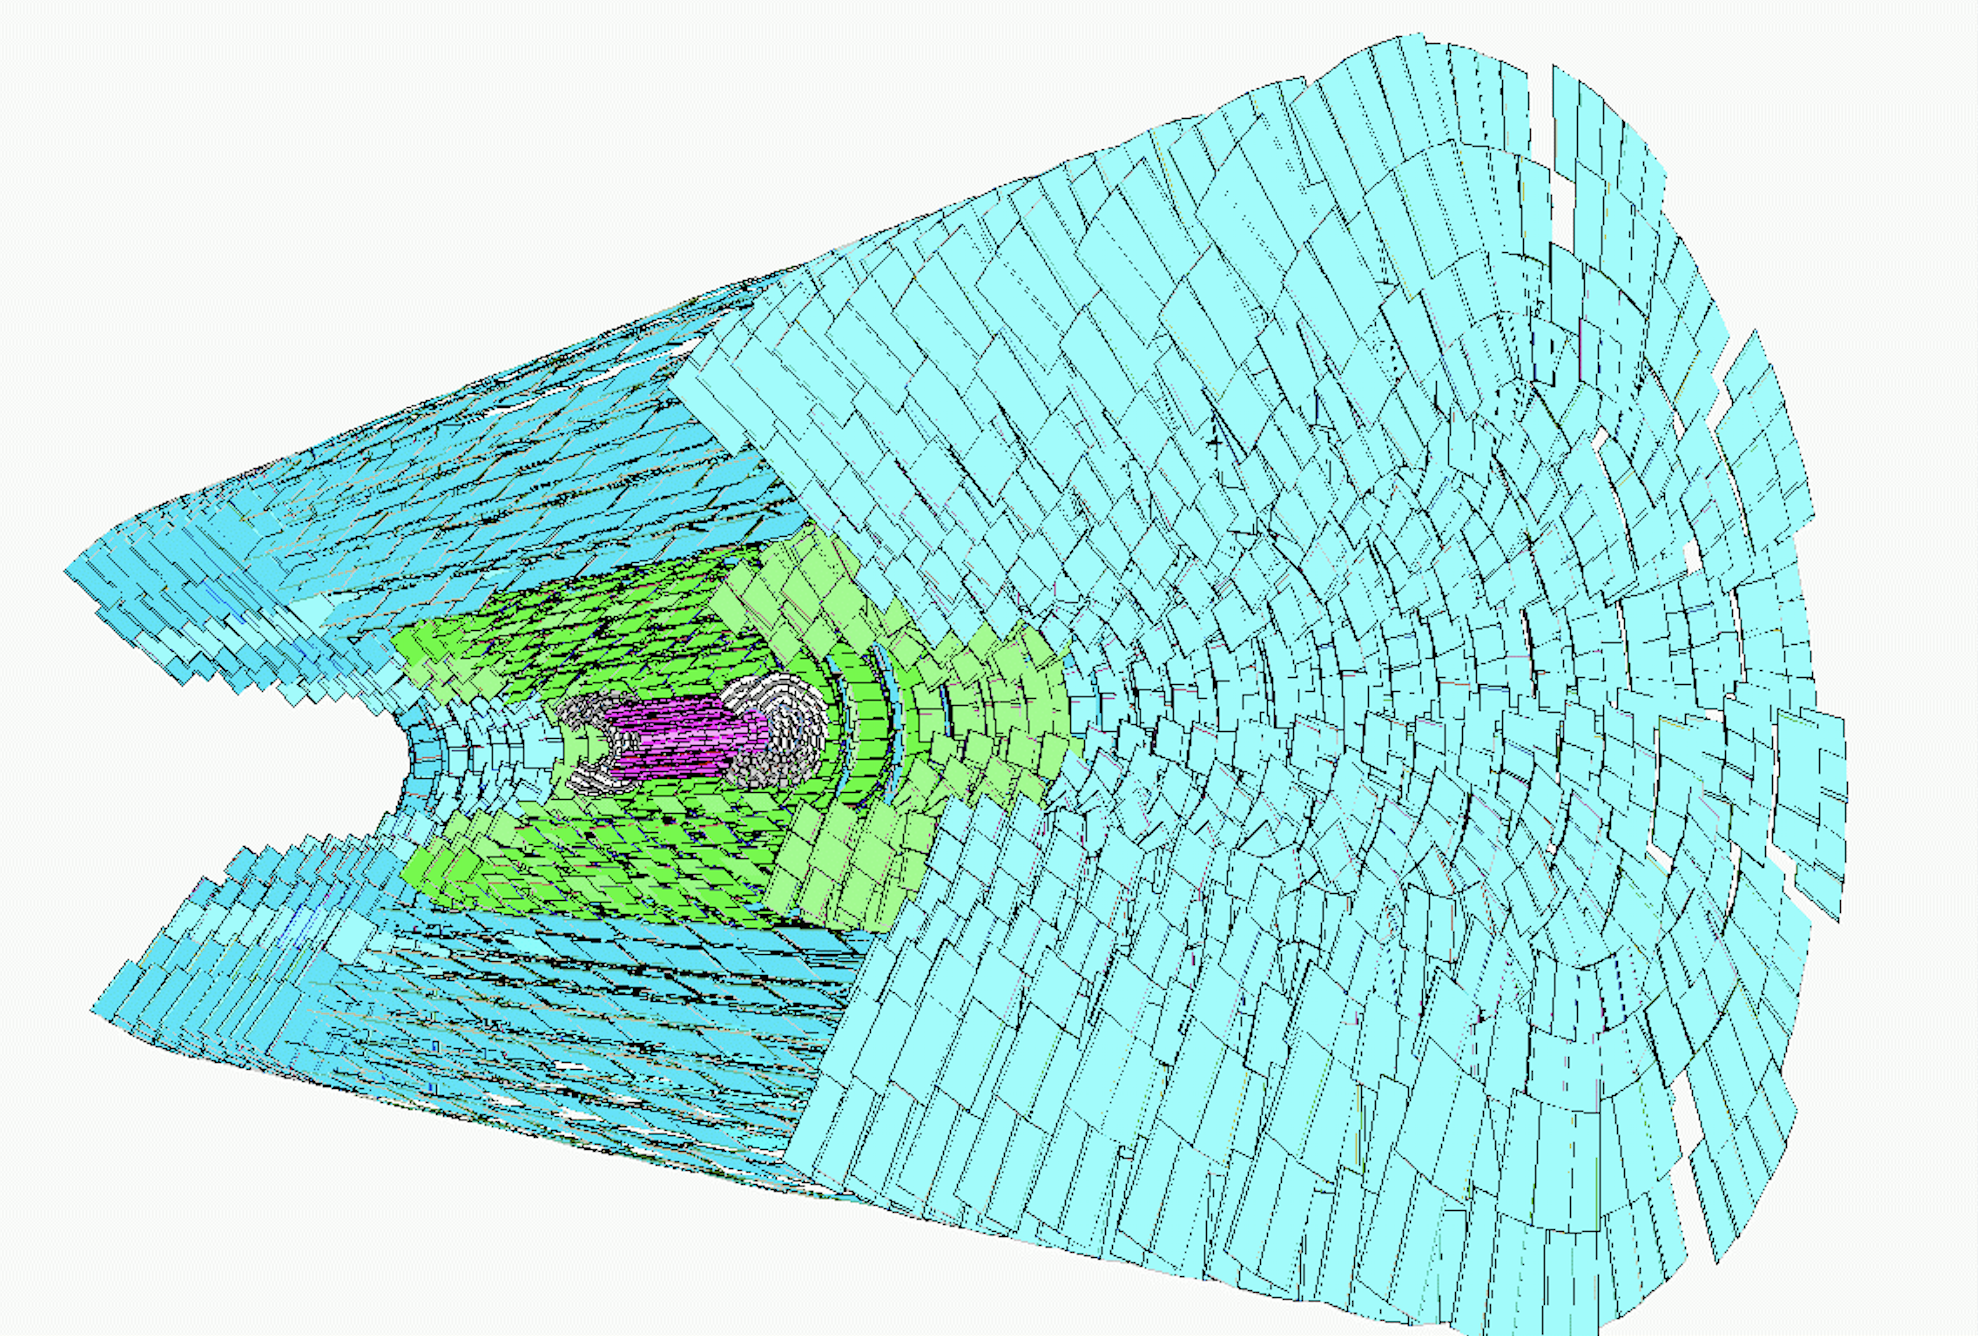
\includegraphics[width=0.49\textwidth,height=10cm,keepaspectratio]{Figures/silicon_tracker_simulated.png}
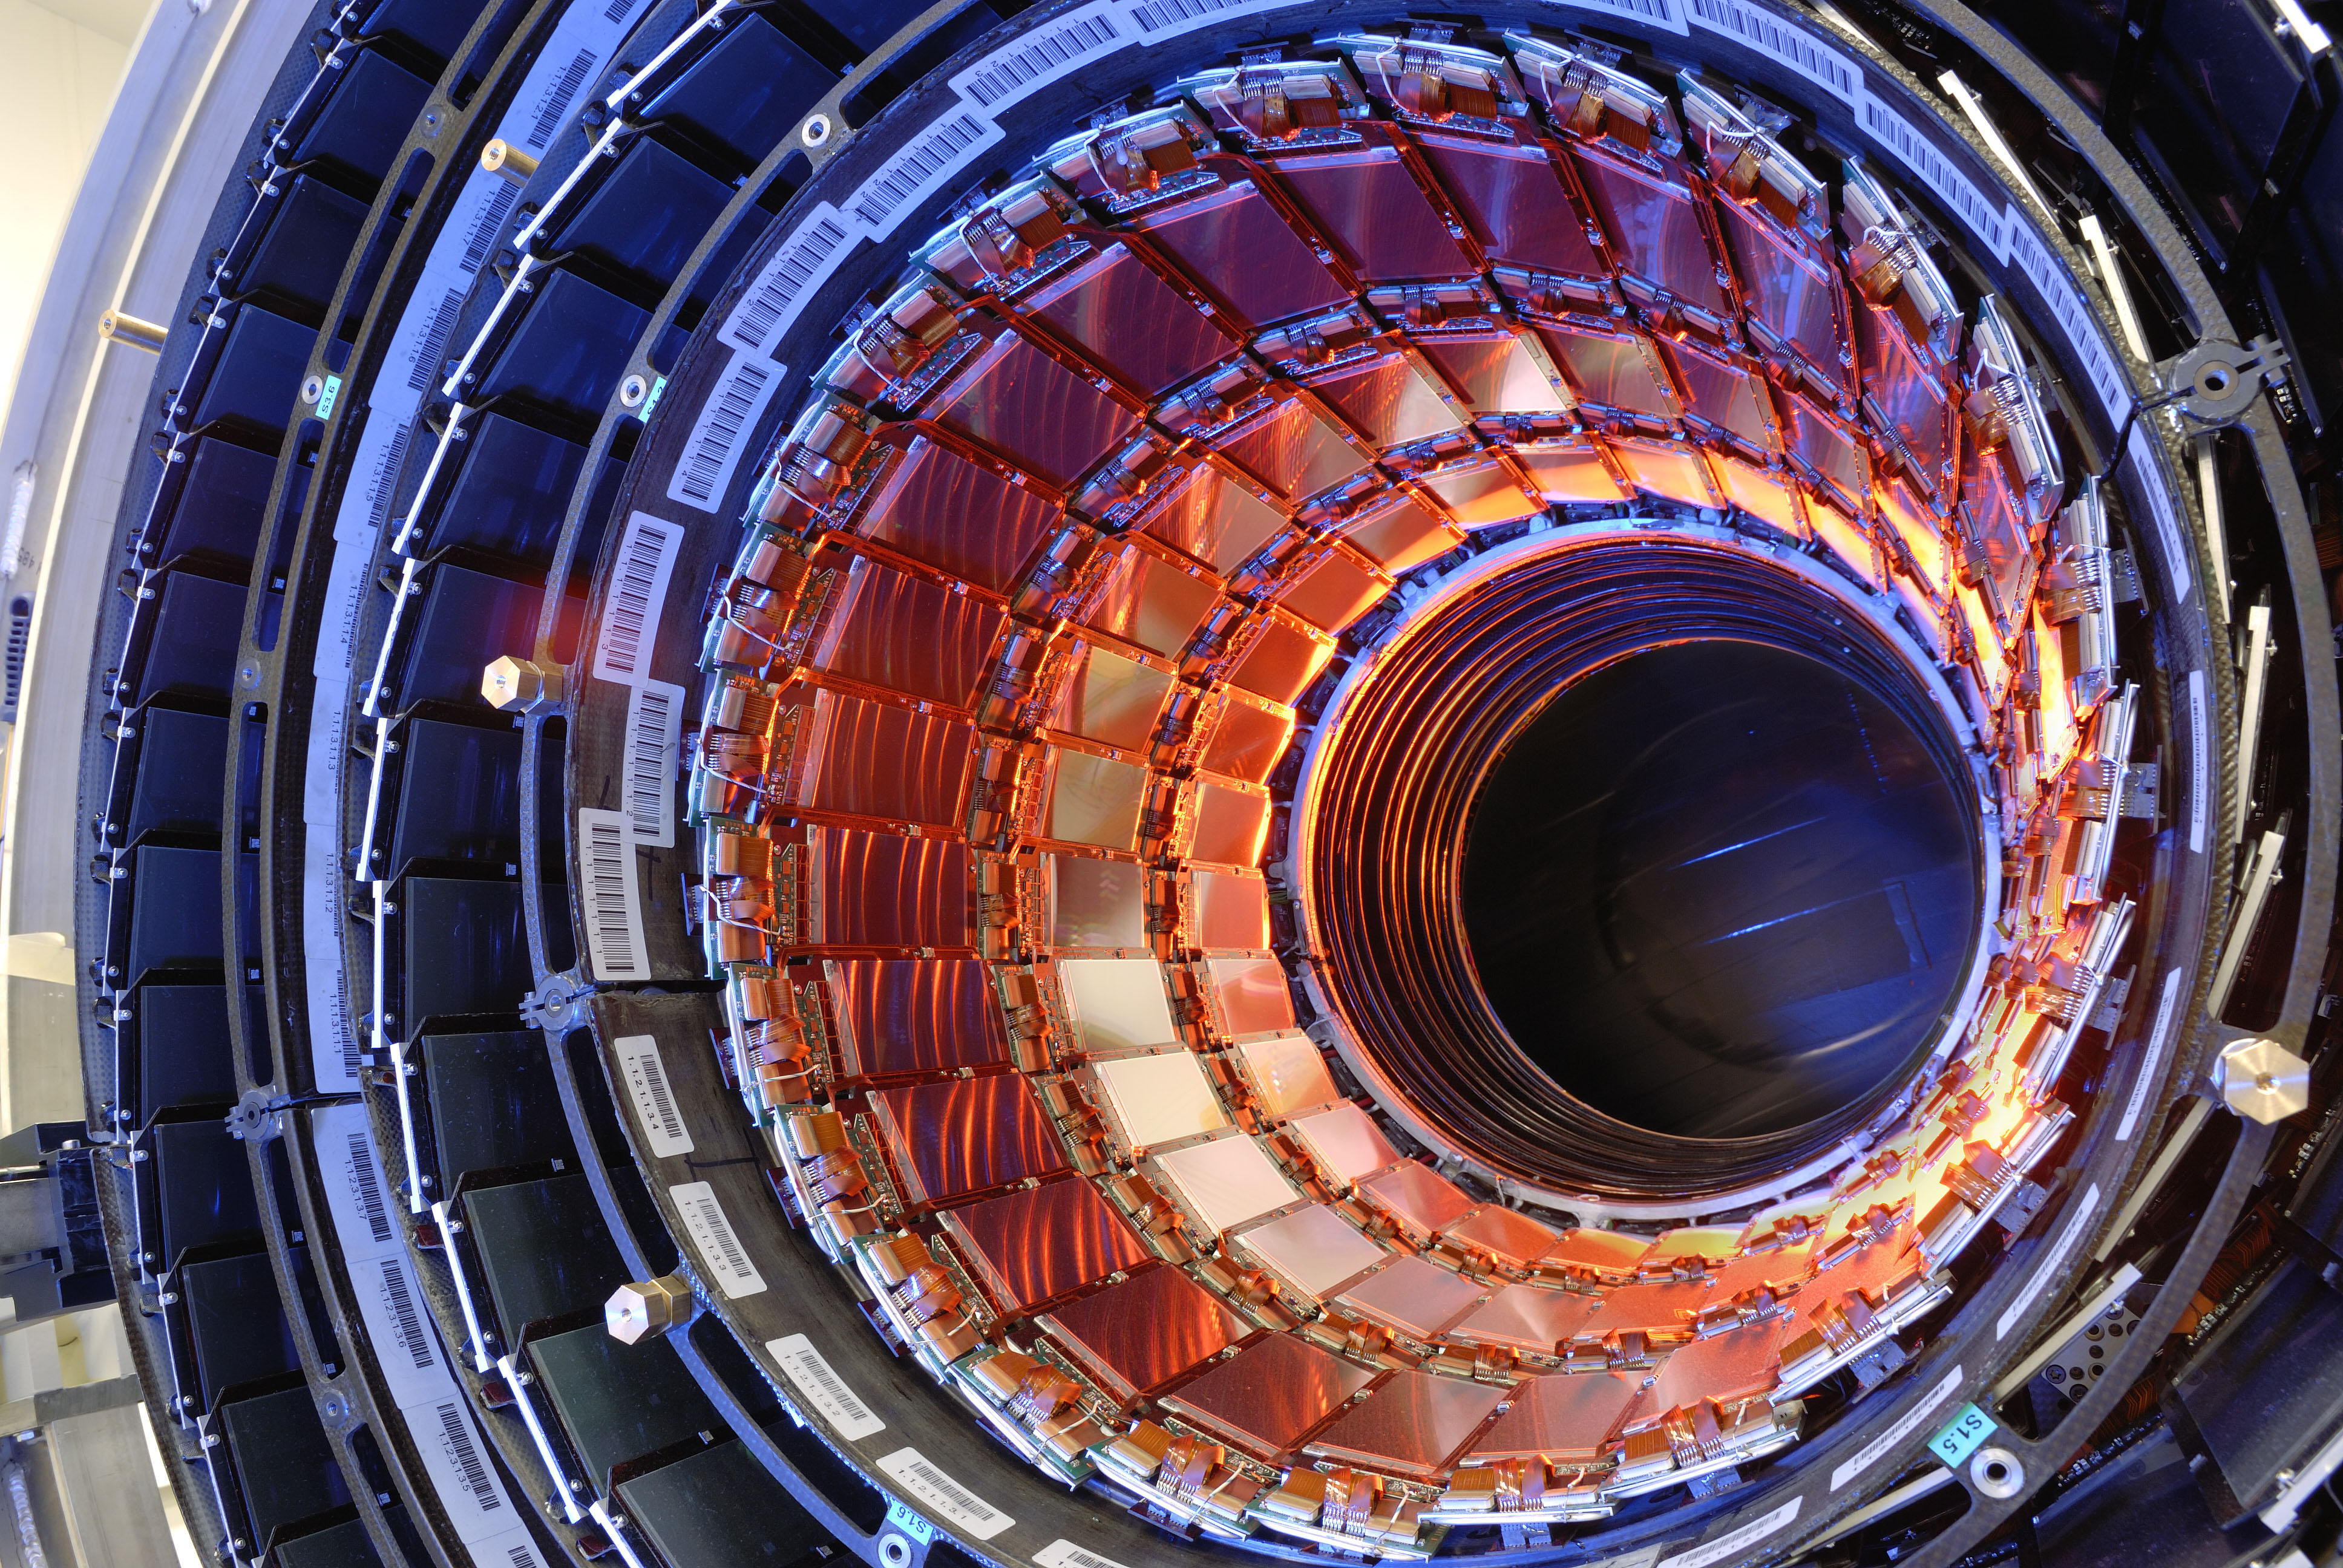
\includegraphics[width=0.49\textwidth,height=10cm,keepaspectratio]{Figures/silicon_tracker_real.jpg}
    \caption{
    (Left) A simulation of the Silicon Tracker, showing the 3 cylindrical layers of the pixel detector (pink), 4 layers of the TIB (green) and the 6 layers of the TOB (blue) of the strip detector.
    The endcap components are also shown.
    (Right) A real picture of the Silicon Tracker. Purdy, isn't it?} 
    \label{fig:tracker_real}
\end{figure}
%%%%%%%%%%%%%%%%%%%%
\begin{figure}[pbth]
\centering
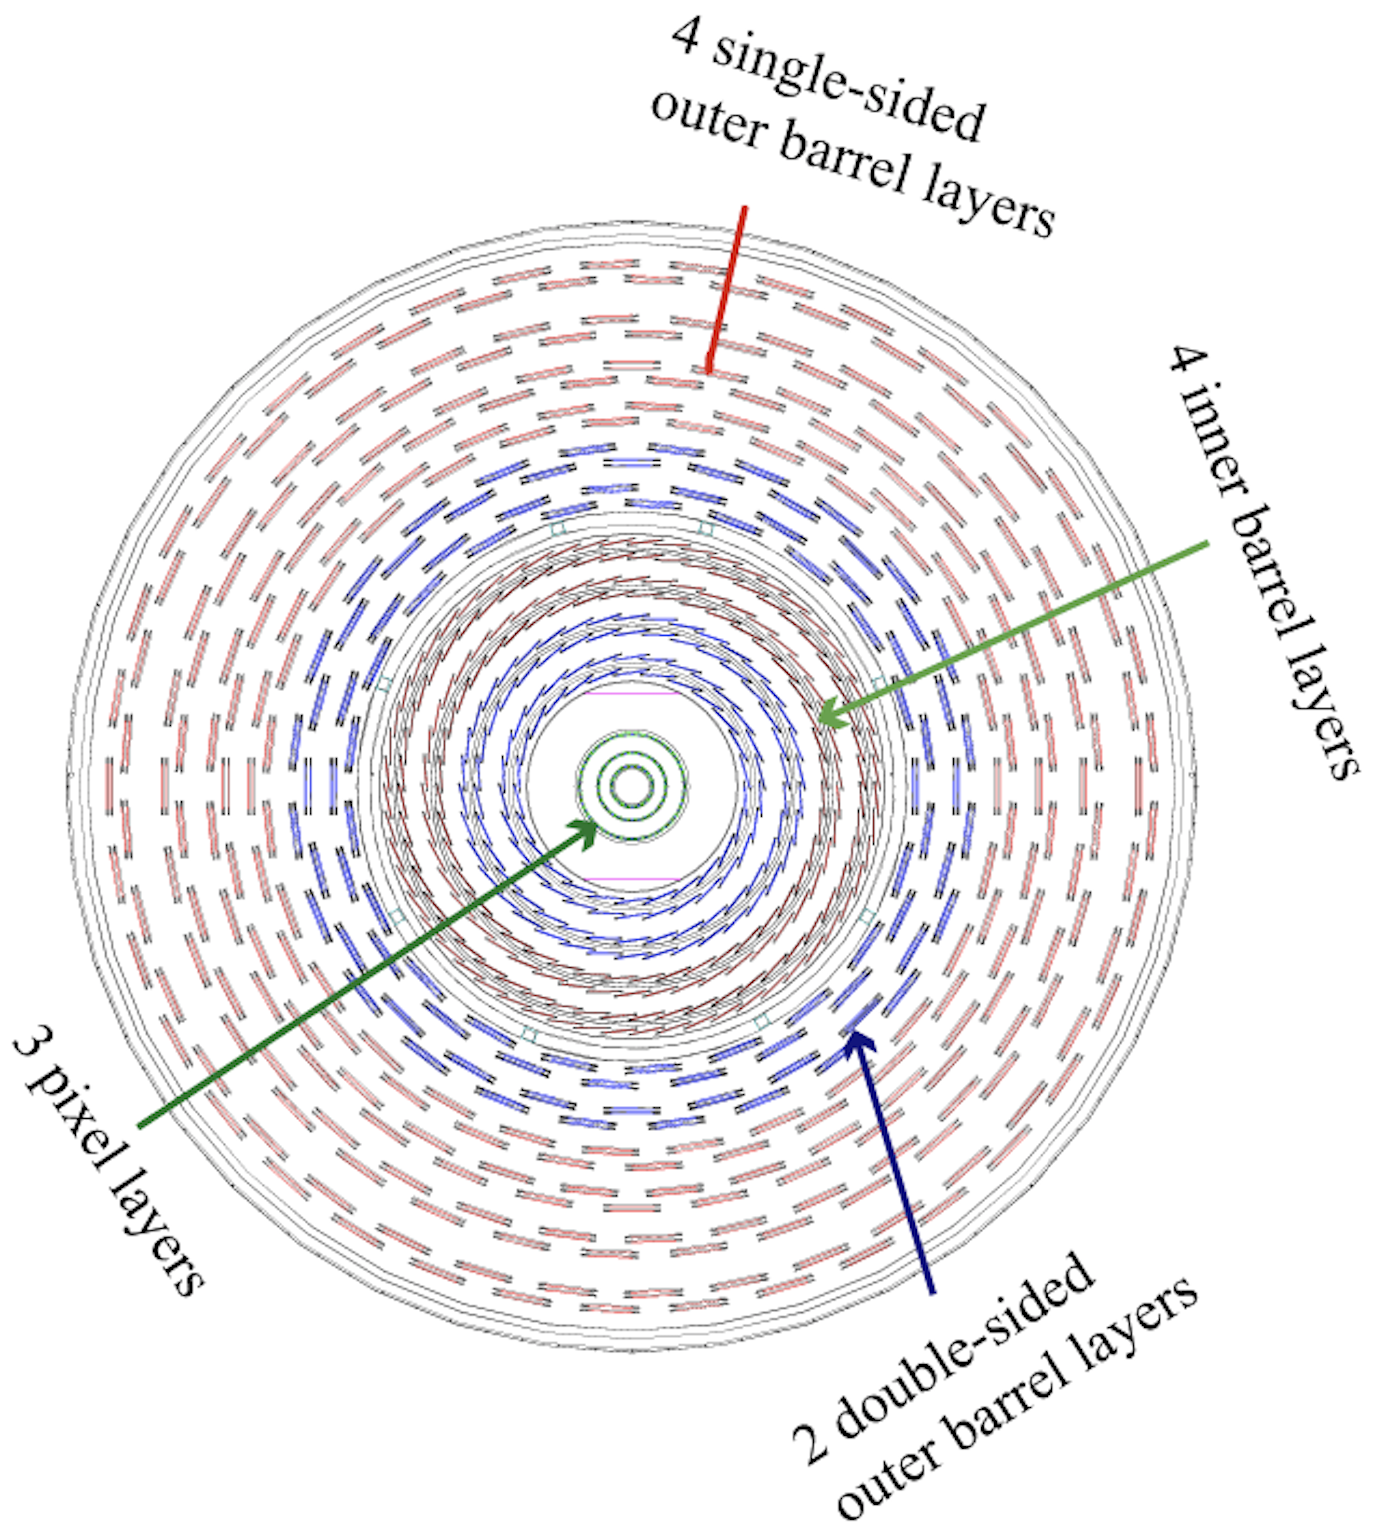
\includegraphics[width=10cm,height=10cm,keepaspectratio]{Figures/silicon_tracker_transverse_view.png}
    \caption{A transverse view of the silicon pixel and strip detectors, explicitly labelling the different layers involved.}
    \label{fig:tracker_xs}
\end{figure}
%%%%%%%%%%%%%%%%%%%%

Consider the life of a particle produced from a $pp$ collision:
Starting at the IP, the produced particles first have an opportunity to interact with the Tracker (Fig.~\ref{fig:tracker_real}, Right).
Only charged particles will generate ``hits'' in the Silicon Tracker.
Therefore, photons, neutrons, and neutral pions, \eg, are invisible to the tracker.
Given enough hits and using sophisticated reconstruction software, we can determine precisely how the particle passed through the tracker.
It's essentially a fancy game of ``connect-the-dots'' to determine the particle's trajectory.
Figuring out the trajectory allows one to measure the radius of curvature, and therefore the momentum of the particle.
This is what makes the Silicon Tracker such an important subdetector.

Another major benefit of the Silicon Tracker is its assistance in vertex identification.
During pile up (multiple proton collisions happening within the same BX),
the tracker can distinguish between proton collisions with a resolution of about 
100 $\mu$m longitudinally and 50 $\mu$m transverse to the beam pipe.
This is crucial to being able to figure out which outgoing particles came from which $pp$ vertex.
Since the tracker wasn't built to catch particles, they usually continue on to the next subsystems.
Thus, CMS must be built as a kind of ``particle filter''.
Electrons and photons are the first to be filtered out by the Electromagnetic Calorimeter...
